\chapter{Event Reconstruction}
\label{evReco}
%a little on daq, event building here?

%Only dealing with parts of event relevant to \Zee analysis.  

The information from the detector for any given event 
gets read out over millions of channels 
from the many different subdetectors.  
These signals must be combined to provide 
meaningful physics information 
%that can be analyzed
about the interaction that took place 
within the detector, 
namely the measurable quantities 
(like direction and energy) 
of the outgoing decay products.  

\section{Detector Object Reconstruction}
\label{evReco:detReco}
%This is for the basic objects only. 
%BUT, basic object reconstruction is so integrated with 
%physics object reconstruction, maybe combine them?

The first step of the particle reconstruction 
involves translating the information from each 
detector channel, 
such as position and electronics signal, 
into useful quantities such as position in 
$\eta$-$\phi$ space and energy or momentum.  
This is done by algorithms 
mapping each individual 
detector cell to its $\eta$-$\phi$ placement 
and calculating its energy, 
which necessarily takes into account 
the position of each cell.  
The second step involves 
connecting information from different channels 
to build up a more complex picture of 
the particles that passed through the detector.  

\subsection{Electromagnetic Calorimeter Reconstruction}
\label{evReco:ECAL}
%\subsection{Electromagnetic Calorimeter Clustering}
%reconstruction of position of energy deposits, 
%rechits and that stuff: digitization, calibration?
% where to go for this stuff?? well, reco principles or
% ecal local reco to start...

The information coming directly from the ECAL 
is read out in terms of each cell's electronics response.  
The ECAL reconstruction algorithms translate this into 
an energy value, which is then calibrated 
according to the cell's energy %as well as its 
and 
$\eta$-position.  
The algorithms also calculate quantities 
relevant to the quality of the deposit, 
in particular whether or not the deposit happened 
at a time consistent with the LHC 
bunch collisions, i.e. if it was ``in time'' or ``out of time''.  
%bunch collisions, i.e. if it was ``in time''.  
This information is especially useful in 
identifying apparent energy deposits that have 
been found to come from the 
%electronics themselves; 
signal-conversion electronics theselves (the transducers); % Wesley
these fake deposits were discovered during 
commissioning and are known as ``ECAL spikes''.  
Since the spikes can imitate energy deposits from 
actual 
%decay products, 
particles, % Wesley
they must be removed from the information used 
to reconstruct electrons and other particles.  
They can be distinguished from real particle deposits 
due to their timing 
as well as the fact that the surrounding crystals 
have no trace of a deposit.  
Therefore, if a high-energy deposit has no or 
very little energy in its neighboring crystals, 
or if its timing is not consistent with a bunch 
crossing, 
it is considered a spike and taken out of the 
reconstruction.  

%\subsubsection{ECAL Spike Removal}
%ALSOOOOO need to talk about spikes and spike removal
%(since that's now automatic, but also wasn't previously. 
%then talk about in event selection, because that was 
%a criterion...? no, because it's not a criterion for 
%e.g. newest datasets)
% HAVEN'T FOUND REFERENCE FOR WHAT'S INCLUDED IN RECO
% except for, like, swiss cross and out of time, is that enough?

%\subsection{Pixel Hits} % need?

\subsection{Track Reconstruction}
\label{evReco:track}
A track is a sequence of hits in the tracker, 
reconstructed to trace the trajectory of a passing 
particle.  
The Kalman Filter algorithm is used by default for CMS tracks, 
but is not good at catching abrupt changes in the 
electron trajectory due to bremsstrahlung.  
Therefore, the Gaussian Sum Filter algorithm 
is used for electrons, 
because it is able to find 
those hits in unexpected directions.  

\subsubsection{Kalman Filter}
\label{evReco:KF}
% CMS Note 2006/041
% CMS Note 2006/026 for seeding
The Kalman Filter (KF) tracking method \cite{CMS-NOTE-2006-041} 
is seeded \cite{CMS-NOTE-2006-026}
by pairs of hits in the pixel detector.  
The seeding algorithm first searches for a hit 
in one of the outer layers of the pixel detector.  
If a hit is found, another hit is sought in a 
layer closer to the interaction point, 
looking in an $\eta$-$\phi$ window around 
the original hit.  
Only two out of the three pixel layers are 
required to have hits 
in order to maintain a high efficiency.  
Once a track seed is found, 
further hits are sought in each successive tracking layer. 
The Kalman filter method is used to predict possible 
locations for hits in the next layer based on 
the currently-known track parameters. % and their 
%uncertainties.  
Hits in that area are then sought and included 
in the track, combining each hit with the 
predicted location for that layer and weighting 
each value depending on the value's uncertainty.  
If there are multiple candidate hits in the next layer, 
a possible trajectory is calculated for each hit, 
along with a trajectory accounting for the case 
in which the hit in that layer was lost.  
This procedure is repeated for each layer: 
each of the calculated trajectories for a given layer 
is matched to hits in the next layer, 
for which new trajectories are calculated.  
To prevent the number of necessary calculations 
from growing too large, 
the number of possible trajectories at each step 
is capped at five.  
%(BUT HOW DETERMINED WHICH ONES???)
%at each layer
In the case of multiple possible trajectories 
for a given fully-reconstructed track, 
defined by two trajectories sharing more than 
half of each of their hits,
the track candidate with fewer hits 
(or, in the case of the same number of hits, 
the track with the worse fit)
is discarded.  

\subsubsection{Gaussian Sum Filter}
\label{evReco:GSF}
% CMS Note 2005/001

The Kalman Filter track-fitting does not accurately 
account for the behavior of particles in a material, 
specifically energy lost in the material 
and changes in direction due to radiation.  
The KF description is in particular inadequate 
for electrons, which 
readily interact with matter in these ways.  
%are prone to these interactions with matter.  
The Gaussian Sum Filter (GSF) algorithm 
\cite{CMS-NOTE-2005-001} was 
therefore developed:
essentially a Kalman Filter 
with a more sophisticated energy loss modeling.   
Instead of approximating the energy loss 
(which is non-Gaussian)
with a Gaussian distribution, 
which KF implicitly does, 
the GSF method models it as a 
weighted sum of Gaussian distributions.  
This greatly improves the performance 
of the track-fitting for electrons.  
%PICTURE? trk-gsf-QoverP.png shows charge-to-momentum
% ratio for KF and GSF -- but figure out 
% WHAT Q/P ACTUALLY TELLS YOU

\section{Electron Reconstruction}
\label{evReco:elec}
% https://twiki.cern.ch/twiki/bin/view/CMS/ElectronRecoPrinciples
% https://twiki.cern.ch/twiki/bin/view/CMS/SWGuideEcalRecoClustering
%here's where we start talking about electrons
%CMS Note 2006/040
As an electron 
%from an interaction 
passes through the CMS detector, 
it leaves a signature pattern in the subdetectors.  
Characteristically, electrons produce a track 
in the tracker system, 
as well as an energy deposit in the 
electromagnetic calorimeter.  
Therefore an electron is reconstructed 
by matching tracks and energy clusters 
that appear to have been made by the same particle 
\cite{CMS-NOTE-2006-040}.  
There are currently two approaches used to 
initiate electron reconstruction: 
the ``ECAL-driven'' method and 
the ``tracker-driven'' method, 
named according to which subdetector's 
information initiates the reconstruction.  
%one starts with ECAL information 
%while the other begins with information from 
%the tracker.  
Each method produces a collection of 
basic electron candidate objects, 
each consisting of a calorimeter cluster 
and hits in the first few layers of the tracker.  
These collections are then combined into one 
and used as seeds to reconstruct the electron tracks, 
producing fully-reconstructed electrons.  
%how many electrons are one vs other vs both?

\subsection{ECAL-driven Electron Seeding}
\label{evReco:ecalDrv}

The ECAL-driven electron reconstruction method 
starts with an energy deposit (or ``supercluster'') 
in the ECAL 
and searches for hits in the 
pixel system that matches the 
position of the calorimeter deposit.  

\subsubsection{Superclusters}
\label{evReco:SC}
%Hybrid and multi5x5 (hybrid doesn't start with basic clusters, 
%so probably combine detector object and physics object sections)

The calorimeter energy deposit used in the electron 
reconstruction is called a supercluster: 
a cluster of clusters.  
A single electron or photon deposits most of its energy 
in a 5x5 square of ECAL crystals, 
as shown in Fig. \ref{fig:BasicCluster}.  
However, an electron passing through the tracker material 
in a strong magnetic field produces 
bremsstrahlung and electrons from converted photons, 
causing the original electron's energy to 
have spread out in $\phi$ once it reaches the calorimeter.  
The process of creating a supercluster gathers these 
energy deposits to form the initial energy of the electron.  

 \begin{figure}[htb]
  \begin{center}
%    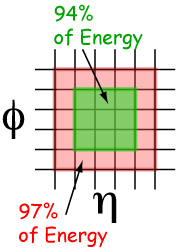
\includegraphics[width=360pt]{Figures/elec-BasicCluster-opaque.png}
    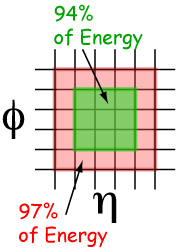
\includegraphics[width=180pt]{Figures/elec-BasicCluster-opaque.png}
  \end{center}
  \caption[\fixspacing Typical energy distribution in a basic cluster]
	  {\fixspacing Typical energy distribution in a basic cluster.}
  \label{fig:BasicCluster}
 \end{figure}

% need pretty picture!

The electron reconstruction currently uses two different 
superclustering methods, 
the ``hybrid'' supercluster method in the barrel, 
and the ``multi5x5'' clustering method in the endcap.  
The hybrid algorithm forms superclusters 
and basic clusters from the same energy deposit 
information, 
while the multi5x5 algorithm first forms 
a single collection of basic clusters, 
which are then separately combined into superclusters.  

%Hybrid
%``hybridSuperClusters''
%hybrid: (dynamic phi road turned OFF)
%http://cmssw.cvs.cern.ch/cgi-bin/cmssw.cgi/CMSSW/RecoEcal/EgammaClusterProducers/python/hybridSuperClusters_cfi.py?revision=1.10&view=markup
%http://cmssw.cvs.cern.ch/cgi-bin/cmssw.cgi/CMSSW/RecoEcal/EgammaClusterProducers/src/HybridClusterProducer.cc?revision=1.32&view=markup
%http://cmssw.cvs.cern.ch/cgi-bin/cmssw.cgi/CMSSW/RecoEcal/EgammaClusterAlgos/src/HybridClusterAlgo.cc?revision=1.61&view=markup


The hybrid algorithm, 
shown in Figure~\ref{fig:HybridSuperCluster}, 
starts with a list of all 
ECAL crystals with an energy greater than a threshold; 
these crystals are considered seeds.  
Beginning with the highest seed crystal, 
the area around each seed is searched for 
energy deposits in steps of one crystal in $\phi$.
For each $\phi$ step, a ``domino'' of crystals is 
formed in $\eta$: 
one crystal to each side of the central crystal, 
or, if the energy sum of those three crystals is 
greater than a threshold, 
two crystals to each side of the central crystal, 
for a total of five crystals per domino.  
The process is done for a given number of $\phi$ 
steps in both the positive and negative directions 
(currently 17 steps).  
As other seeds are encountered in this process, 
they are removed from the list of available seeds.  
Each domino with a higher energy than its two neighbors 
is considered as the seed for a basic cluster, 
and the collection of dominos formed by the search 
process is the basis for the supercluster.  
The basic clusters are formed by summing the 
energy of each local-maximum domino with 
those of its neighboring lower-energy dominos, 
excluding dominos that have already been used.  
The supercluster is then formed by summing the energies 
of the constituent basic clusters, 
with its seed considered to be the highest-energy 
basic cluster 
and its position given by the energy-weighted positions 
of the constituent clusters.  

 \begin{figure}[htb]
  \begin{center}
    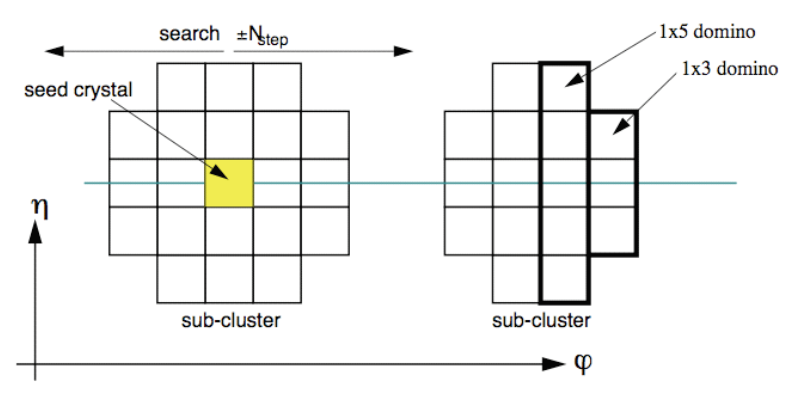
\includegraphics[width=360pt]{Figures/elec-SC-hybrid-algo.png}
  \end{center}
  \caption[\fixspacing Illustration of the ``Hybrid'' supercluster algorithm]
	  {\fixspacing Illustration of the ``Hybrid'' supercluster algorithm. 
	    Dominoes with energy above a given threshold are constructed 
	    along the $\phi$ direction in both directions out from the seed crystal.  
	  }
  \label{fig:HybridSuperCluster}
 \end{figure}



%Multi5x5:
%``multi5x5SuperClustersWithPreshower''

%https://twiki.cern.ch/twiki/bin/view/CMS/ECALDPGClusterization  also talks about supercluster energy corrections
%http://cmssw.cvs.cern.ch/cgi-bin/cmssw.cgi/CMSSW/RecoEcal/EgammaClusterProducers/python/multi5x5SuperClusters_cfi.py?revision=1.2&view=markup
%http://cmssw.cvs.cern.ch/cgi-bin/cmssw.cgi/CMSSW/RecoEcal/EgammaClusterProducers/src/Multi5x5ClusterProducer.cc?revision=1.5&view=markup
%http://cmssw.cvs.cern.ch/cgi-bin/cmssw.cgi/CMSSW/RecoEcal/EgammaClusterAlgos/src/Multi5x5ClusterAlgo.cc?revision=1.9&view=markup
%http://cmssw.cvs.cern.ch/cgi-bin/cmssw.cgi/CMSSW/RecoEcal/EgammaClusterProducers/src/Multi5x5SuperClusterProducer.cc?revision=1.2&view=markup
%http://cmssw.cvs.cern.ch/cgi-bin/cmssw.cgi/CMSSW/RecoEcal/EgammaClusterAlgos/src/Multi5x5BremRecoveryClusterAlgo.cc?revision=1.8&view=markup SCORE

The multi5x5 algorithm, 
shown in Figure~\ref{fig:Multi5x5SuperCluster}, 
first creates a collection 
of basic clusters from seeds, 
which are ECAL crystals with an energy higher than 
a given threshold.  
If a seed represents a local maximum, 
then its energy deposit is combined with those 
from the crystals in the surrounding 5x5 square 
to form a basic cluster, 
ignoring any crystals that have already been 
used to form the central 3x3 part of another cluster.  
The basic clusters are then used as seeds for the 
superclustering algorithm.  
For each seed cluster with energy higher than a threshold, 
the energies of any other clusters within an $\eta$-$\phi$ 
window of the seed (longer in $\phi$ than in $\eta$)
are combined with its own energy to create the supercluster, 
leaving out clusters that have already been used to 
form another supercluster. 
The position of the supercluster is given by the 
energy-weighted position of the individual clusters.  

 \begin{figure}[htb]
  \begin{center}
    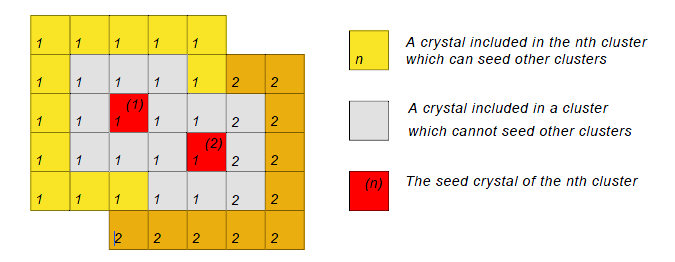
\includegraphics[width=360pt]{Figures/elec-SC-multi5x5-algo.png}
  \end{center}
  \caption[\fixspacing Illustration of the ``Multi5x5'' supercluster algorithm]
	  {\fixspacing Illustration of the ``Multi5x5'' supercluster algorithm.
	    Clusters seeded by seed crystals are grouped into 
	    superclusters.  
	  }
  \label{fig:Multi5x5SuperCluster}
 \end{figure}



%also preshower cluster info in endcap... how?
%what kind of energy corrections done? 
%or is that for energy scale section?
%at least SC corrections are in dpg clusterization twiki

\subsubsection{Pixel Hit-matching}
\label{evReco:pixMatch}

To reconstruct the full electron, 
the supercluster must be matched with a track.  
% where exactly to split ecal-driven and tracker-driven?
This is done by extrapolating the probable position of 
tracker hits from the supercluster's position, 
%given the supercluster energy.  
as illustrated in Fig. \ref{fig:PixMatch}.  
Given the supercluster energy and the fact that a 
non-radiating electron would have hit the calorimeter 
at the energy-weighted center of the supercluster's 
energy spread, 
the electron's initial (pre-radiation) trajectory 
through the tracker can be calculated 
for both the positive and negative electron 
charge cases.  
The reconstruction algorithm then looks for a matching 
hit in the first pixel detector layer 
within a $\phi$-$z$ window of this position 
for each charge case.  
If a hit is found, another hit is sought in the second 
pixel layer within a different $\phi$-$z$ window 
of the hit in the first layer.  
%This set of pixel hits is the seed(??)

%PICTURE from my old talk or something!  

 \begin{figure}[htb]
  \begin{center}
%    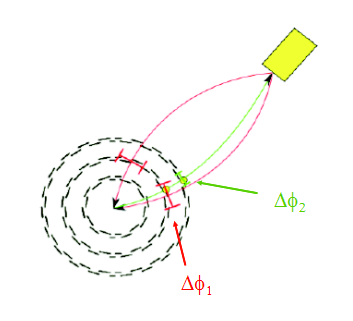
\includegraphics[width=360pt]{Figures/elec-pixmatch.png}
    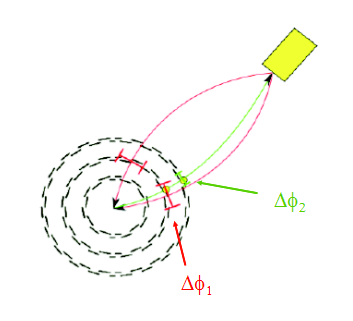
\includegraphics[width=240pt]{Figures/elec-pixmatch.png}
  \end{center}
  \caption[\fixspacing Schematic of pixel-hit search algorithm in electron-seeding]
	  {\fixspacing Schematic of pixel-hit search algorithm in electron-seeding. 
	    For both the positive and negative electron charge cases, 
	    a possible trajectory is extrapolated back from the calorimeter deposit 
	    given the deposit's energy. 
	    A hit is sought along either trajectory in either the inner or 
	    middle pixel layer within a window ($\Delta\phi_1$). 
	    If a hit is found, a second hit is sought along that trajectory 
	    in the next pixel layer(s) ($\Delta\phi_2$).}
  \label{fig:PixMatch}
 \end{figure}

\subsection{Tracker-driven Electron Seeding}
\label{evReco:trkDrv}
% AN 2008/032 michele pioppi
In the tracker-driven electron seeding method, 
electron-finding is seeded by tracks, 
which are followed out to the 
ECAL to search for calorimeter clusters 
associated with each track.  
This method was developed to better deal with 
low-\pT electrons, for which the energy deposits 
from bremsstrahlung may be too widely separated 
to be matched,  
and non-isolated electrons within jets, 
whose energy deposits are not necessarily 
distinguishable from those of surrounding hadrons.  
For these electrons the calorimeter cluster-based 
seeding does not perform as well as for 
isolated, high-\pT electrons.  

The tracker-driven electron seeding method 
takes as input the default collection 
of tracks, obtained by an iterative usage 
of the KF algorithm.  
The method first tries to follow each track 
all the way to the calorimeter and search 
for nearby energy clusters.  
All clusters with an acceptable E/p ratio 
with respect to the track are tested, 
and the cluster closest in $\eta$-$\phi$ 
space to the track is the one chosen. 
 
Out of the tracks that were not 
well associated to any energy cluster, 
a preselection is applied to select 
those tracks that may have resulted from 
radiating electrons, 
which would not have been found 
by the cluster-matching method.  
If the track was not matched because it had 
too few tracker hits and could not be traced 
to the calorimeter, 
or if the KF algorithm did not fit the 
track well enough because of possible 
bremsstrahlung, the tracks are passed 
on to the next step of the selection.  
A reduced GSF track-fitting algorithm 
is then run on these tracks, 
in an attempt to recover the 
bremsstrahlung-induced changes in track direction. 
This reduced version of the GSF algorithm runs 
much faster than that with the default parameters, 
but the performance is slightly reduced.  

Finally, a multi-variate analysis (MVA) using 
boosted decision trees 
is performed on these candidates.  
The MVA algorithm is 
%trained 
calibrated 
on a sample of electrons from 
$b \bar{b}$ events, which are primarily non-isolated, 
and a sample of \Zee events, 
which provides high-\pT electrons.  
%List of MVA variables?: ...
The output of the MVA is a number indicating 
the likelihood of the object being an electron.   
Those objects whose MVA output is greater than a threshold 
are considered electron candidates. 
These candidates are then combined with those 
previously identified from the cluster-matching 
to produce the final collection of 
tracker-driven electron seeds.  

\subsection{Electron Track Reconstruction}
\label{evReco:elecTrk}

The full collection of electron seeds, 
both ECAL- and tracker-driven, 
are used as the basis for reconstructing 
the electron track and hence 
completing the electron reconstruction.  
As mentioned previously, 
the electron reconstruction uses the 
GSF algorithm to reconstruct tracks.  
The electron kinematics are 
assigned to be a weighted combination 
of those of the constituent supercluster 
and track, 
and the final electron collection 
is saved for further analysis.  

%%%%%%%\subsection{Z Reconstruction}

%\subsection{Electron Energy Scale and Resolution} %???

%\subsection{Electron Isolation Variables} %???? here, or in electron selection????
%\subsection{Electron Identification Variables} %???? again, here????

\section{Beam Spot Reconstruction}
\label{evReco:BS}
%maybe include just to talk about primary vertex correction
% https://twiki.cern.ch/twiki/bin/view/CMSPublic/SWGuideFindingBeamSpot
% cms note 2007/021
The region where the beams overlap and protons may interact, 
the ``luminous region'', is called the beam spot.  
Typically this area is a few centimeters long, 
with a width of 20-50 microns.  % Wesley
The beam spot location can be used as an estimate 
for the initial position of tracks measured in the detector, 
and is therefore useful in track-seeding.  
Its position %and width %how? necessary?
%in all three dimensions %how is it done for z?
can be determined from measurements of tracks in the 
general track collection 
\cite{CMS-NOTE-2007-021}.  
%This is done by applying a fit to the distance of 
%the tracks' closest approach to the nominal beam spot (0,0,0), 
%plotted as a function
This is done by making a distribution of each track's distance of 
closest approach to the nominal beam spot (0,0,0) 
as a function of the track's $\phi$ angle at its 
closest approach.  
If the beam spot is far from (0,0,0), 
the distribution looks sinusoidal.  
This distribution is then fit with a sine curve 
parametrized in the beam spot's actual 
$x$- and $y$-positions, 
and these values are extracted.  
Initially, one beam spot position was calculated    % Wesley (I think this is what he wanted)
for a full run.  
The calculation switched to using smaller run segments 
called ``luminosity sections'' (LS) 
in order to account for changes in the beam spot position 
during a run.  

\section{Primary Vertex Reconstruction} % ? probably
\label{evReco:PV}
% few twikis with some info (most don't have much):
% https://twiki.cern.ch/twiki/bin/view/CMSPublic/WorkBookVertexReco
% https://twiki.cern.ch/twiki/bin/view/CMSPublic/SWGuideVertexReco
% https://twiki.cern.ch/twiki/bin/view/CMSPublic/WorkBookOfflinePrimaryVertexFinding
% http://twiki.cern.ch/twiki/bin/view/CMSPublic/SWGuideOfflinePrimaryVertexProduction has like the most info
% possibly cms note 2006/026 section 7 (reference in kf paper) using pixels for pv reco
% also cms note 2006/029, section 3.1 - vertex finding

Since protons may collide anywhere within the region of 
beam overlap, 
the main interaction in a given event may not necessarily 
happen at the exact center of the detector.  
In particular, there may be a significant displacement 
in the $z$-direction.  
Determining the location of the main interaction, 
also called the primary vertex, 
is an integral part of reconstructing the event.  
For example, an electron may leave a deposit in 
a given calorimeter cell that has a fixed $\eta$ position 
relative to the nominal interaction point, 
the very center of the detector (0,0,0).  
However, if the interaction producing the electron 
actually takes place at a different point, 
the electron's actual $\eta$ position will be 
different relative to the interaction.  
Therefore the position of the primary vertex 
should be taken into account when calculating $\eta$.  

% GENERAL PROCESS FOR VERTICES, BUT PV SIMPLE CASE!(?)
%The process of reconstructing the primary vertex consists 
%of two steps: vertex-finding and vertex-fitting.  
%In the first step primary vertex candidates 
%are created from the tracks in the event, 
%matching each track to the interaction 
%that likely produced it.  
%In the second, 
%the resulting vertices are fit and examined 
%to determine various parameters, 
%like the goodness of the fit to the vertex.  
%BLAH, fix if actually need
%ACTUALLY, PV reco does some fitting anyhow, 
%looks like it's already in ``pv-finding'' algo
%as described in that cms note

The process of the reconstructing the primary vertex 
\cite{CMS-NOTE-2006-026}, 
\cite{CMS-NOTE-2006-029} 
involves creating primary vertex candidates
from the tracks in the event,
matching each track to the interaction
that likely produced it.
This is done by grouping the tracks according 
to their $z$-position at the point at which they pass 
most closely to the beam spot.  
The tracks are required to pass relatively close 
to the beamline, 
and they are also required to have a \pt greater 
than some threshold (with a default of 1.5 GeV).  
Tracks within a small distance (default 1 mm) of each other 
at the beam spot are considered to have come from 
the same vertex, 
and the primary vertex candidates are formed from these 
groups of tracks.  
At this point a fit is applied to each primary vertex candidate, 
and tracks found to be incompatible with the candidate are discarded 
until all tracks meet a given compatibility level.  
Finally, vertices that are incompatible with the position 
of the beam spot are discarded.  
(A second algorithm uses the beam spot as constraint on the 
position of the vertex fit itself, 
but this algorithm was not fully commissioned at the time 
of this study.)  
If no reconstructed primary vertex candidates are found in 
an event, 
a ``fake'' primary vertex is added at the position 
of the beam spot.  
Since more than one interaction per event is possible 
but generally only one is of interest (the ``primary'' interaction), 
multiple candidates are ordered according to transverse energy of 
their constituent tracks, 
and the highest of these is taken to be the primary vertex.  

\clearpage
